\section{Comparison to StochasticSplats}
\label{app:stocSplats}

\begin{table*}[t]
    \caption{\label{tab:ssplats_benchmarks}
        \textbf{Novel view synthesis}: Comparison between our method, our method with stochastic forward pass, and \cite{kv2025stochasticsplats}, in terms of both speed and quality.
    }
    \centering
    \small
    \begin{threeparttable}
        \footnotesize % or \footnotesize for slightly larger text
        \setlength{\tabcolsep}{4.2pt} % reduce horizontal padding between columns
        \begin{tabular}{
            l
            S[table-format=2.2] S[table-format=1.3] S[table-format=1.3] l
            S[table-format=2.2] S[table-format=1.3] S[table-format=1.3] l
            S[table-format=2.2] S[table-format=1.3] S[table-format=1.3] l
        }
        \toprule
        \multirow{2}{*}{Method\textbackslash Metric}
         & \multicolumn{4}{c}{\textbf{MipNeRF360}} 
         & \multicolumn{4}{c}{\textbf{Tanks \& Temples}}
         & \multicolumn{4}{c}{\textbf{Deep Blending}} \\
        \cmidrule(lr){2-5} \cmidrule(lr){6-9} \cmidrule(lr){10-13}
         & {PSNR$\uparrow$} & {SSIM$\uparrow$} & {LPIPS$\downarrow$} & {Time$\downarrow$}
         & {PSNR$\uparrow$} & {SSIM$\uparrow$} & {LPIPS$\downarrow$} & {Time$\downarrow$}
         & {PSNR$\uparrow$} & {SSIM$\uparrow$} & {LPIPS$\downarrow$} & {Time$\downarrow$} \\
        \midrule
        %Ours           & 28.05 & 0.852 & 0.251   & {} & {} & {} & {} & {} & {} & {} & {} \\
        \textbf{Ours}     & 28.31 & 0.857 & 0.254 & 33m & 22.57 & 0.830 & 0.221 & 20m & 29.87 & 0.906 & 0.324 & 25m \\
        \textbf{Ours-FullStoch} (15spp)     & 27.90 & 0.843 & 0.265 & 37m & 22.37 & 0.821 & 0.233 & 21m & 29.51 & 0.902 & 0.330 & 24m \\
        \textbf{Ours-Fullstoch} (30spp)     & 28.14 & 0.850 & 0.254 & 52m & 22.75 & 0.827 & 0.229 & 25m & 29.75 & 0.904 & 0.327 & 29m \\
        \textbf{SS-Tracing}  & 22.12 & 0.648 & 0.451 & 89m & 14.94 & 0.532 & 0.560 & 54m & 18.08 & 0.726 & 0.578 & 68m \\
        %Stoch-Splats   & 24.67 & 0.714 & 0.392 & {1h23m23s} & {} & {} & {} & {} & {} & {} & {} & {} \\
        \bottomrule
        \end{tabular}
    \end{threeparttable}
\end{table*}

Proposed by \citet{kv2025stochasticsplats}, StochasticSplats introduces a stochastic method for estimating gradients of the alpha-blended pixel colors $C$ with respect to the Gaussian parameters.
%Although StochasticSplats uses rasterization (instead of ray tracing), their gradient estimator could be adopted as an alternative of ours expressed in Algorithm~2 of the main paper.
In what follows, we present the pseudo-code for the alternative estimator in \autoref{alg:ssplats}, and compare the efficiency of both estimators via empirical experiments.

\begin{algorithm}[t]
    \caption{\label{alg:ssplats}
        Monte Carlo estimator for pixel color gradient $\dCdbalpha$ introduced by StochasticSplats~\cite{kv2025stochasticsplats}.
    }
    %
	\SetCommentSty{mycmtfn}
	\SetKwComment{tccinline}{// }{}
    %
    % $\dCdbcEst \gets \boldsymbol{0}$; 
    $\dCdbalphaEst^\mathrm{ssplats} \gets \boldsymbol{0}$\;
    \For{$m = 1$ to $\Mb$}{
        \tcc{Draw index $I$}
        $I \gets 0$; $z \gets \infty$; $\alpha \gets 1$\;
        \ForEach{Gaussian $g_i$ along the camera ray}{ 
            Obtain its opacity $\alpha_i$ and depth $z_i$\;
            Draw $\xi$ uniformly from $[0, 1)$\;
            \If{$\xi < \alpha_i$ and $z_i < z$}{
                $I \gets i$; $z \gets z_i$; $\alpha \gets \alpha_i$\; 
                
            }
        }
        %
        \If{$I > 0$}{
            \tcc{Obtain Gaussian color}
            Compute the color $c_I$ of the Gaussian $g_I$\; 
            \ForEach{Gaussian $g_k$ along the camera ray}{
                Obtain its opacity $\alpha_k$ and depth $z_k$\;
                \If{$z_k < z_I$}{
                    \tcc{Update the gradient estimates}
                    $\dCdbalphaEst^\mathrm{ssplats}_k \pluseq \nicefrac{-c_I}{(1 - \alpha_k)}$
                        \label{line:div_by_zero}
                        \tccinline*{\autoref{Eq:ssplats_dCdbalpha_1}}
                }
            }            
            \tcc{Update the gradient estimates}
            % $\dCdbcEst_I \pluseq 1$ \tccinline*{\autoref{Eq:ssplats_dCdbc}}
            $\dCdbalphaEst^\mathrm{ssplats}_I \pluseq \nicefrac{c_I}{\alpha}$
                \tccinline*{\autoref{Eq:ssplats_dCdbalpha_0}}
        }
    }
    %
    \Return %$\nicefrac{\dCdbcEst}{\Mb}$, 
        $\nicefrac{\dCdbalphaEst^\mathrm{ssplats}}{\Mb}$\;
\end{algorithm}

\subsection{Alternative Gradient Estimator}
\label{ssec:ssplats_grad_est}

StochasticSplats~\cite{kv2025stochasticsplats} uses the same procedure as our method to estimate the gradient $\dCdbc$ but a different one for $\dCdbalpha$.
In the following, we focus on the estimation of the latter.

As described in \autoref{alg:ssplats}, to estimate the gradient $\dCdbalpha := (\nicefrac{\partial C}{\partial\alpha_1}, \nicefrac{\partial C}{\partial\alpha_2}, \ldots, \nicefrac{\partial C}{\partial\alpha_n})$ with respect to the Gaussian opacities $\alpha_1, \alpha_2, \ldots, \alpha_n$, StochasticSplats starts with drawing an index $I$ the same way as our method, and setting
%
\begin{equation}
    \label{Eq:ssplats_dCdbalpha_0}
    \dCdbalphaEst^\mathrm{ssplats}_I = \frac{c_I}{\alpha_I}.
\end{equation}
%
Then, instead of randomly drawing some $K \succ I$, StochasticSplats lets
%
\begin{equation}
    \label{Eq:ssplats_dCdbalpha_1}
    \dCdbalphaEst^\mathrm{ssplats}_k = \frac{-c_I}{1 - \alpha_k},
\end{equation}
%
%\sz{In this equation, should the color term be $c_I$ or $c_k$?}
for all Gaussians $g_k$ located in front of the Gaussian $g_I$ (i.e., with $k \prec I$).

Although this approach returns denser gradient estimates by spatting gradients to not only the $I$-th component but also all $k \prec I$, it suffers from two major drawbacks.
First, when executed on the GPU, writing to all $k \prec I$ components in parallel requires significantly more atomic operations, which can lead to reduced computational efficiency.
Second, the division by $(1 - \alpha_k)$ in \autoref{Eq:ssplats_dCdbalpha_1} can produce near-infinite gradients---and therefore high variance---whenever high-opacity Gaussians make $\alpha_k \approx 1$, which occurs frequently.

\begin{figure*}[t]
    \setlength{\resLen}{1.5in}
    %
    \centering
    \small
    \addtolength{\tabcolsep}{-5.5pt}
    %
    %
    \begin{tabular}{cc}
        % &
        (a) \textbf{Forward} & (b) \textbf{Opacity Values Along the Ray}
        \\
        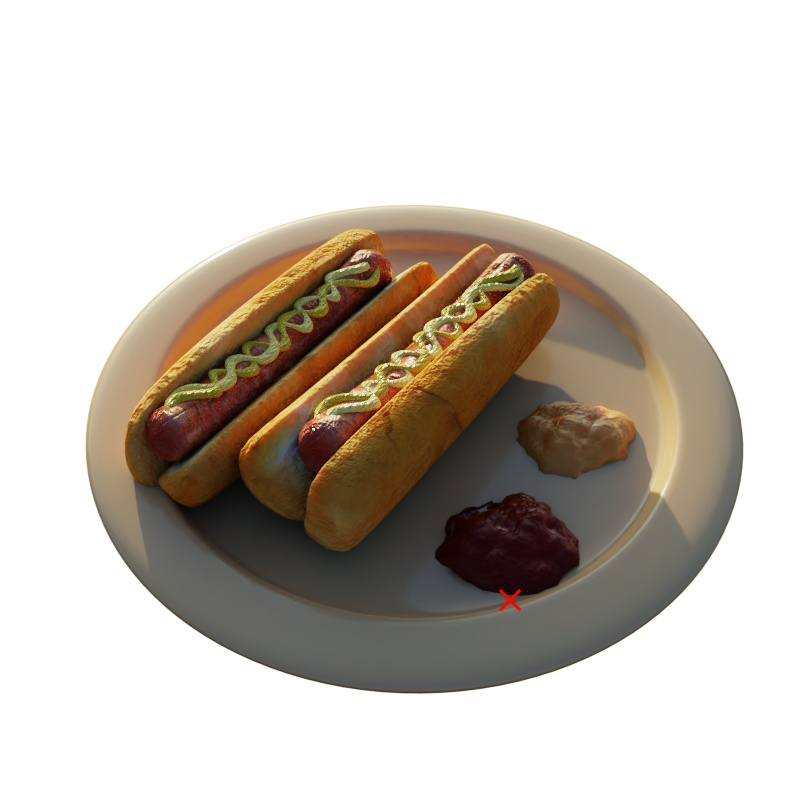
\includegraphics[trim={30 0 30 100}, clip, width=\resLen]{images/grad_image/forward_mark.jpg} &
        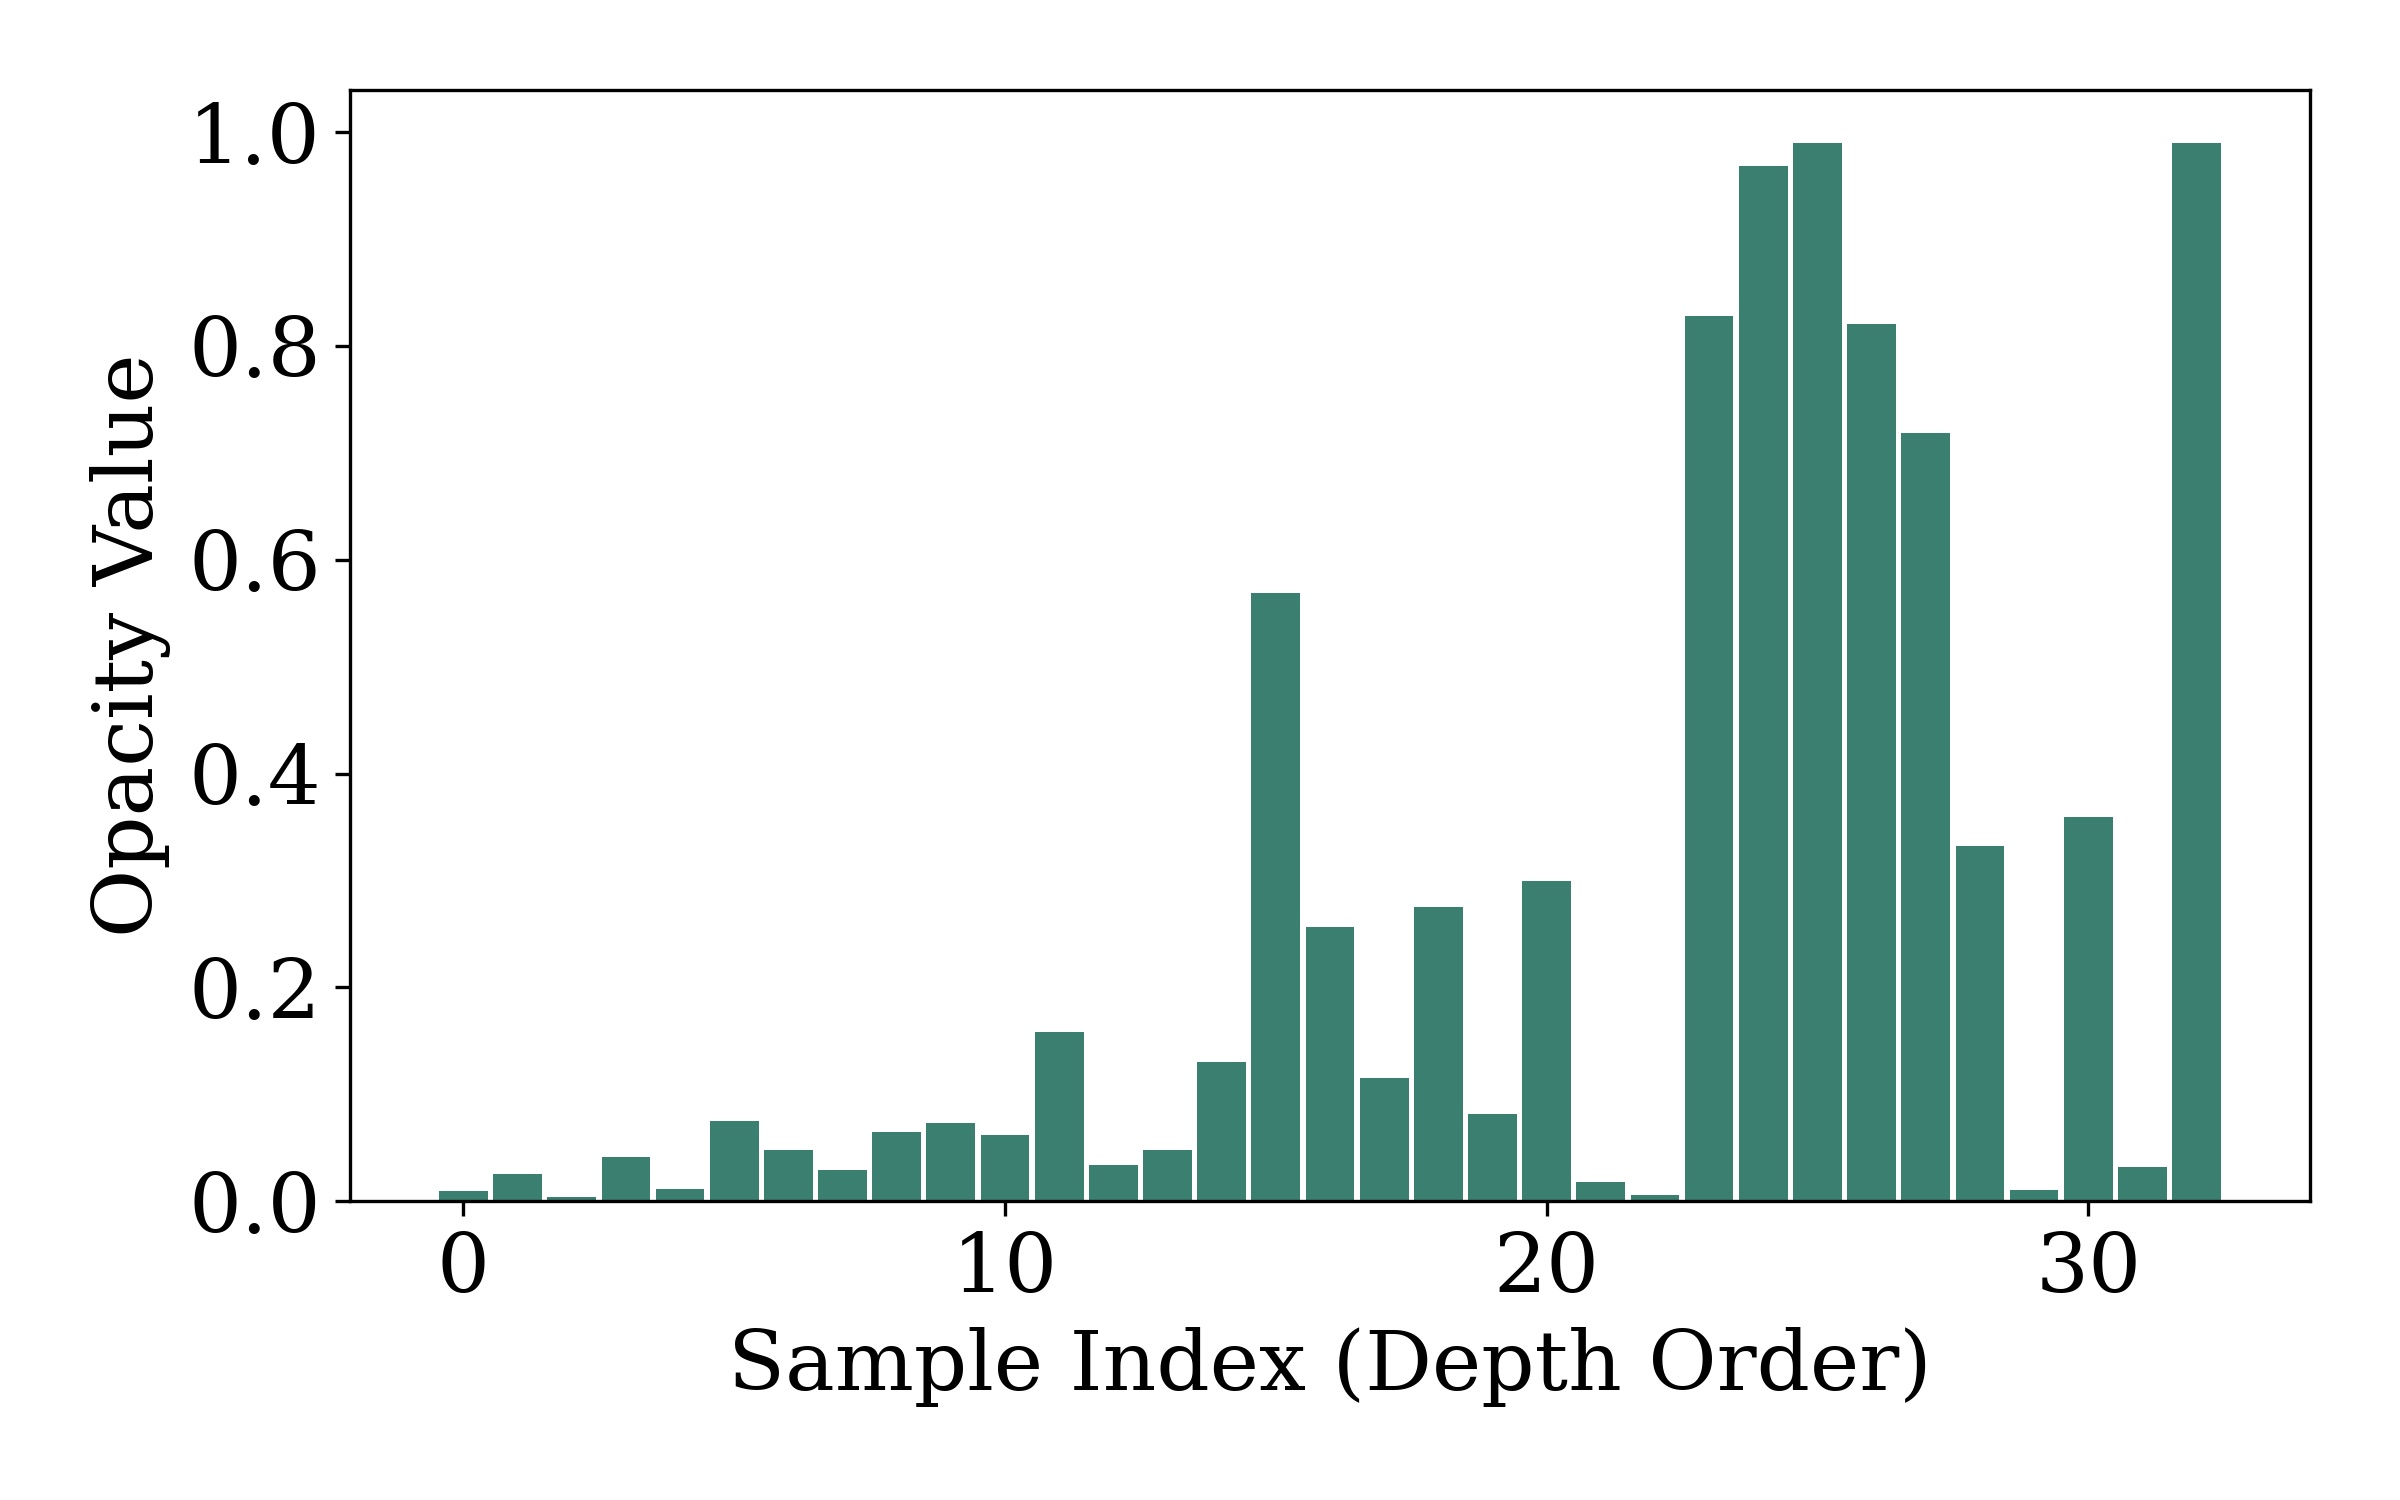
\includegraphics[height=\resLen]{images/grad_image/alpha_histogram.jpg}
    \end{tabular}
    \begin{tabular}{cccc}
        % &
        (c) \textbf{Sorted} & (d) \textbf{Ours, $M_b=8$}  & (e) \textbf{SS-Tracing, $M_b=8$}  & (f) \textbf{SS-Tracing, $M_b=128$}
        \\
        \begin{overpic}[trim={30 0 30 100}, clip, width=\resLen]{images/grad_image/AB.jpg}
            \put(50, 0){\makebox(0,0){\color{black}{\scriptsize \textbf{Time: 21.46ms}}}}
        \end{overpic} &
        \begin{overpic}[trim={30 0 30 100}, clip, width=\resLen]{images/grad_image/ours_8spp.jpg}
            \put(50, 0){\makebox(0,0){\color{black}{\scriptsize \textbf{Time: 10.87ms | RMSE: 0.408}}}}
        \end{overpic} &
        \begin{overpic}[trim={30 0 30 100}, clip, width=\resLen]{images/grad_image/ssplats_8spp.jpg}
            \put(50, 0){\makebox(0,0){\color{black}{\scriptsize \textbf{Time: 28.22ms | RMSE: 1.432}}}}
        \end{overpic} &
        \begin{overpic}[trim={30 0 30 100}, clip, width=\resLen]{images/grad_image/ssplats_128spp.jpg}
            \put(50, 0){\makebox(0,0){\color{black}{\scriptsize \textbf{Time: 484.04ms | RMSE: 0.427}}}}
        \end{overpic}
    \end{tabular}
    %
    \caption{
        Visualization of the variance of the gradient obtained by our method and the baseline method. (a) shows the forward rendering result, and (b) visualizes the opacities of each Gaussian along the ray at the red cross in (a). We further visualize the gradient that the Gaussians along each pixel receive when applying: (c) Sorted alpha blending (3DGRT), (d) Ours, with $M_b=8$, (e) Our implementation of~\cite{kv2025stochasticsplats}, with $M_b=8$, and (f) Our implementation of~\cite{kv2025stochasticsplats}, with $M_b=128$. The time for the backward pass and RMSE are provided with each image.
    }
    \label{fig:gradient_image}
\end{figure*}




The key difference between our method and \cite{kv2025stochasticsplats} is the order of derivation. StochasticSplats~\cite{kv2025stochasticsplats} first designs a Monte Carlo estimator for alpha blending, and subsequently takes the derivative of the estimator. Our method, in contrast, first takes the derivative of alpha blending, and designs a Monte Carlo estimator for the derivative. This ordering introduces a term $\nicefrac{1}{1-\alpha_{K\prec I}}$ in the density gradient, where the denominator easily evaluates to a near-$0$ value when an opaque Gaussian exists, causing problematic gradients.


\subsection{Comparisons}
\label{ssec:ssplats_comp}
%
To compare the efficiency of our gradient estimator (Algorithm~2 of the main paper) and the alternative one proposed by StochasticSplats (\autoref{alg:ssplats}), we implement the latter on our stochastic ray tracing codebase, which we refer to as \textsl{SS-Tracing}.

%\sz{Need to discuss \autoref{fig:gradient_image} here.}
We give an intuition on the variance of both methods in \autoref{fig:gradient_image} by visualizing the gradient image. The images show the magnitude of screen space gradient with respect to the horizontal motion of the Gaussians, as well as a plot of the opacities of Gaussians along a ray. Our experiment shows that high opacity Gaussians frequently occur, and can easily lead to large variance for \textsl{SS-Tracing}. Empirically, it takes $16\times$ samples for SS-Tracing to reach the same level of variance as our method. 


% We show the visual quality in \autoref{fig:benchmark_ssplats}, and the numerical metrics in \autoref{tab:ssplats_benchmarks}.


% For comparison, we implement the StochasticSplats algorithm under the our code framework, referred to as \textbf{SS-Tracing}, and evaluate the reconstruction quality under the same dataset used in Section 5.1 of the main paper. 
We compare the numerical metrics of our method and our re-implemented \textsl{SS-Tracing} in \autoref{tab:ssplats_benchmarks}.